\begin{titlepage}
\begin{center}

\includegraphics[scale=0.15]{Documents/niser.png}
\line(1,0){300}\\
[2mm]
\begin{large}
\textbf{\huge Boolean Logical Operations}\\ 
\end{large}
\line(1,0){150}\\
[5cm]
\large MAITREY SHARMA\\
\small (1911093)\\
[4.5cm]
Second Year Integrated M.Sc.\\
\textbf{School of Physical Sciences}\\
\textbf{National Institute of Science Education and Research, Bhubaneshwar}\\
\small March 17, 2021
\end{center} 
\end{titlepage}
\newpage
\section{Aim}
\noindent To study and verify various Boolean logic operations and the De Morgan’s 
laws using digital ICs.
\section{Apparatus}
\noindent Digital ICs 7404, 7400, 7408, 7432, 7486 and 7402, resistors, DC voltage source of $\SI{5}{\volt}$, LEDs, breadboard and connecting wires.
\section{Theory}
\noindent The integrated circuit which was use for operational amplifier circuit is primarily designed for performing analogue computations. \textbf{\emph{Analogue electronics}} are electronic systems with a continuously variable signal. \textbf{\emph{Digital electronics}} is a field of electronics involving the study of digital signals, where data as a sequence of discrete values in contrast with analogue electronics. For this, digital integrated circuits are employed here which are basically large assemblies of \textbf{\emph{logic gates}}. A logic gate is an idealized model of computation or physical electronic device implementing a \textbf{\emph{Boolean function}}, a logical operation performed on one or more binary inputs that produces a single binary output.
\par
\noindent There are various types of logic families of monolithic digital ICs consisting of logic gates like resistor-transistor logic, diode-transistor logic, transistor-transistor logic etc. The IC7400 series is based on the \textbf{\emph{transistor-transistor logic (TTL)}}. When using a standard $\SI{+5}{\volt}$ supply any TTL voltage input between $\SI{2.0}{\volt}$ and $\SI{5}{\volt}$ is considered to be a logic "1" or "HIGH" while any voltage input below $\SI{0.8}{\volt}$ is recognized as a logic "0" or "LOW". TTL outputs are typically restricted to narrower limits of between $\SI{0}{\volt}$ and $\SI{0.4}{\volt}$ for a "low" and between $\SI{2.7}{\volt}$ and $\SI{5}{\volt}$. The voltage region between the maximum voltage of logic “0” and minimum voltage of logic “1” of either input or output is called the \textbf{\emph{intermediate region}}.
\begin{center}
    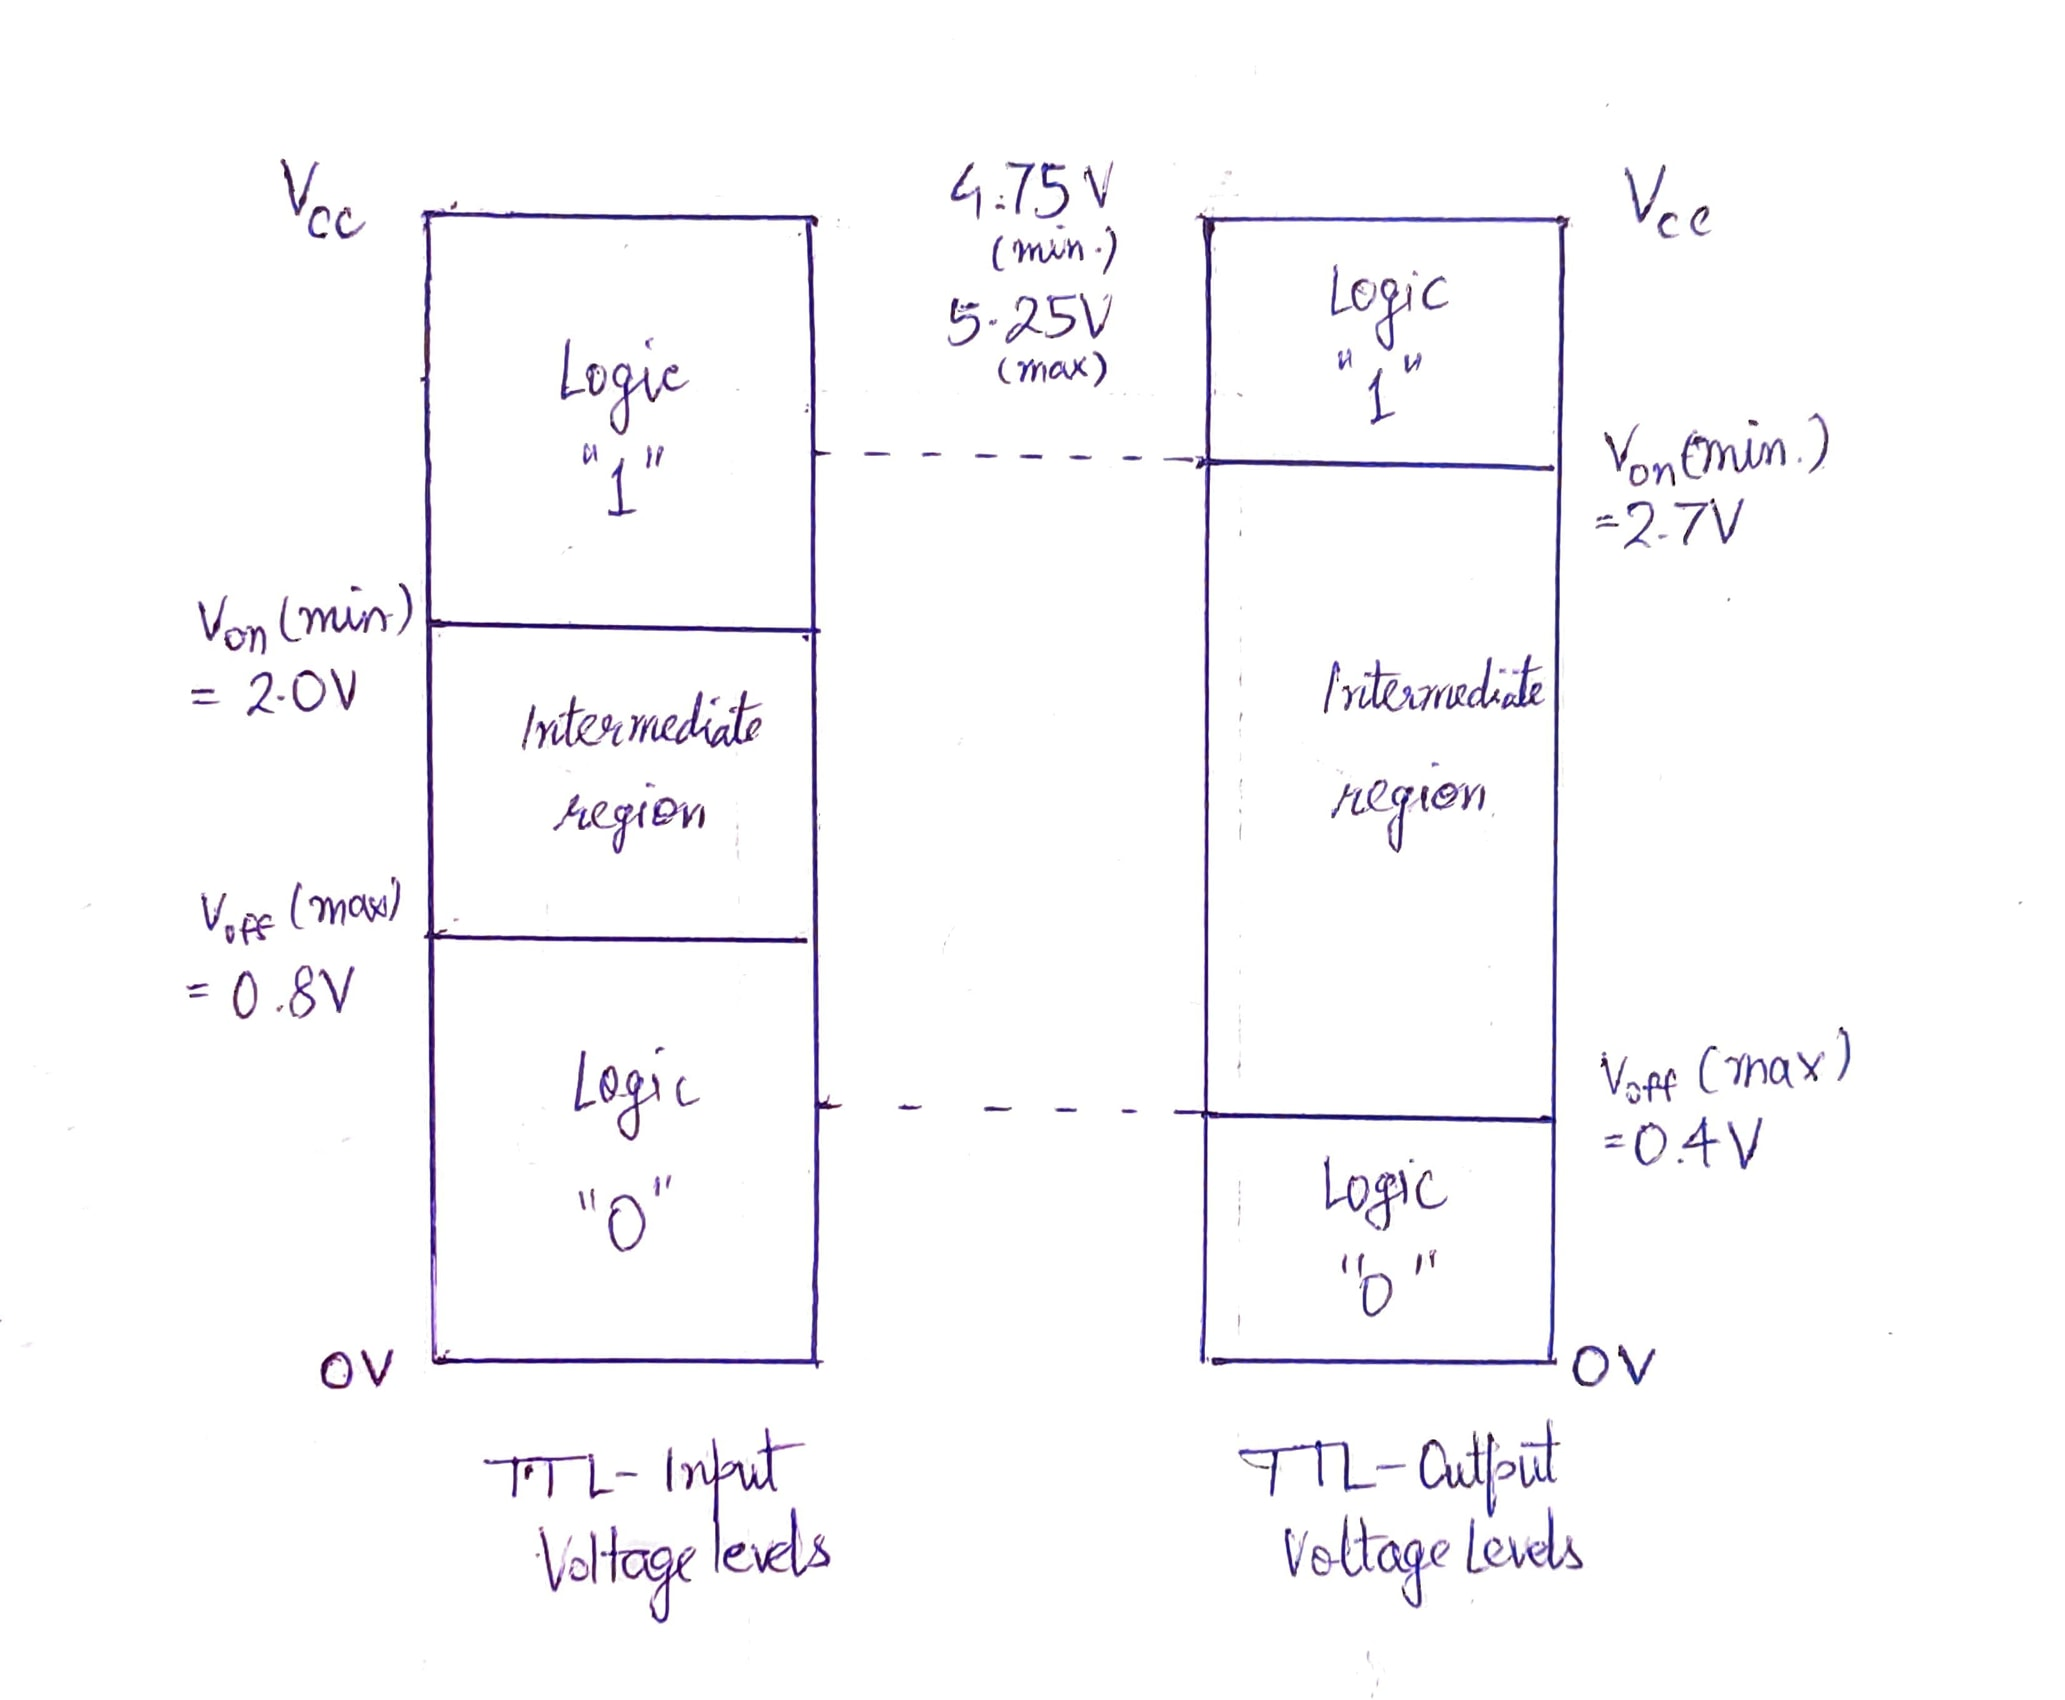
\includegraphics[scale = 0.16]{Documents/1615791787718.jpg}
\end{center}
\clearpage
\noindent
There are several types of logic gates as shown below. We will construct the truth-tables for each one as part of our experiment.
\begin{center}
    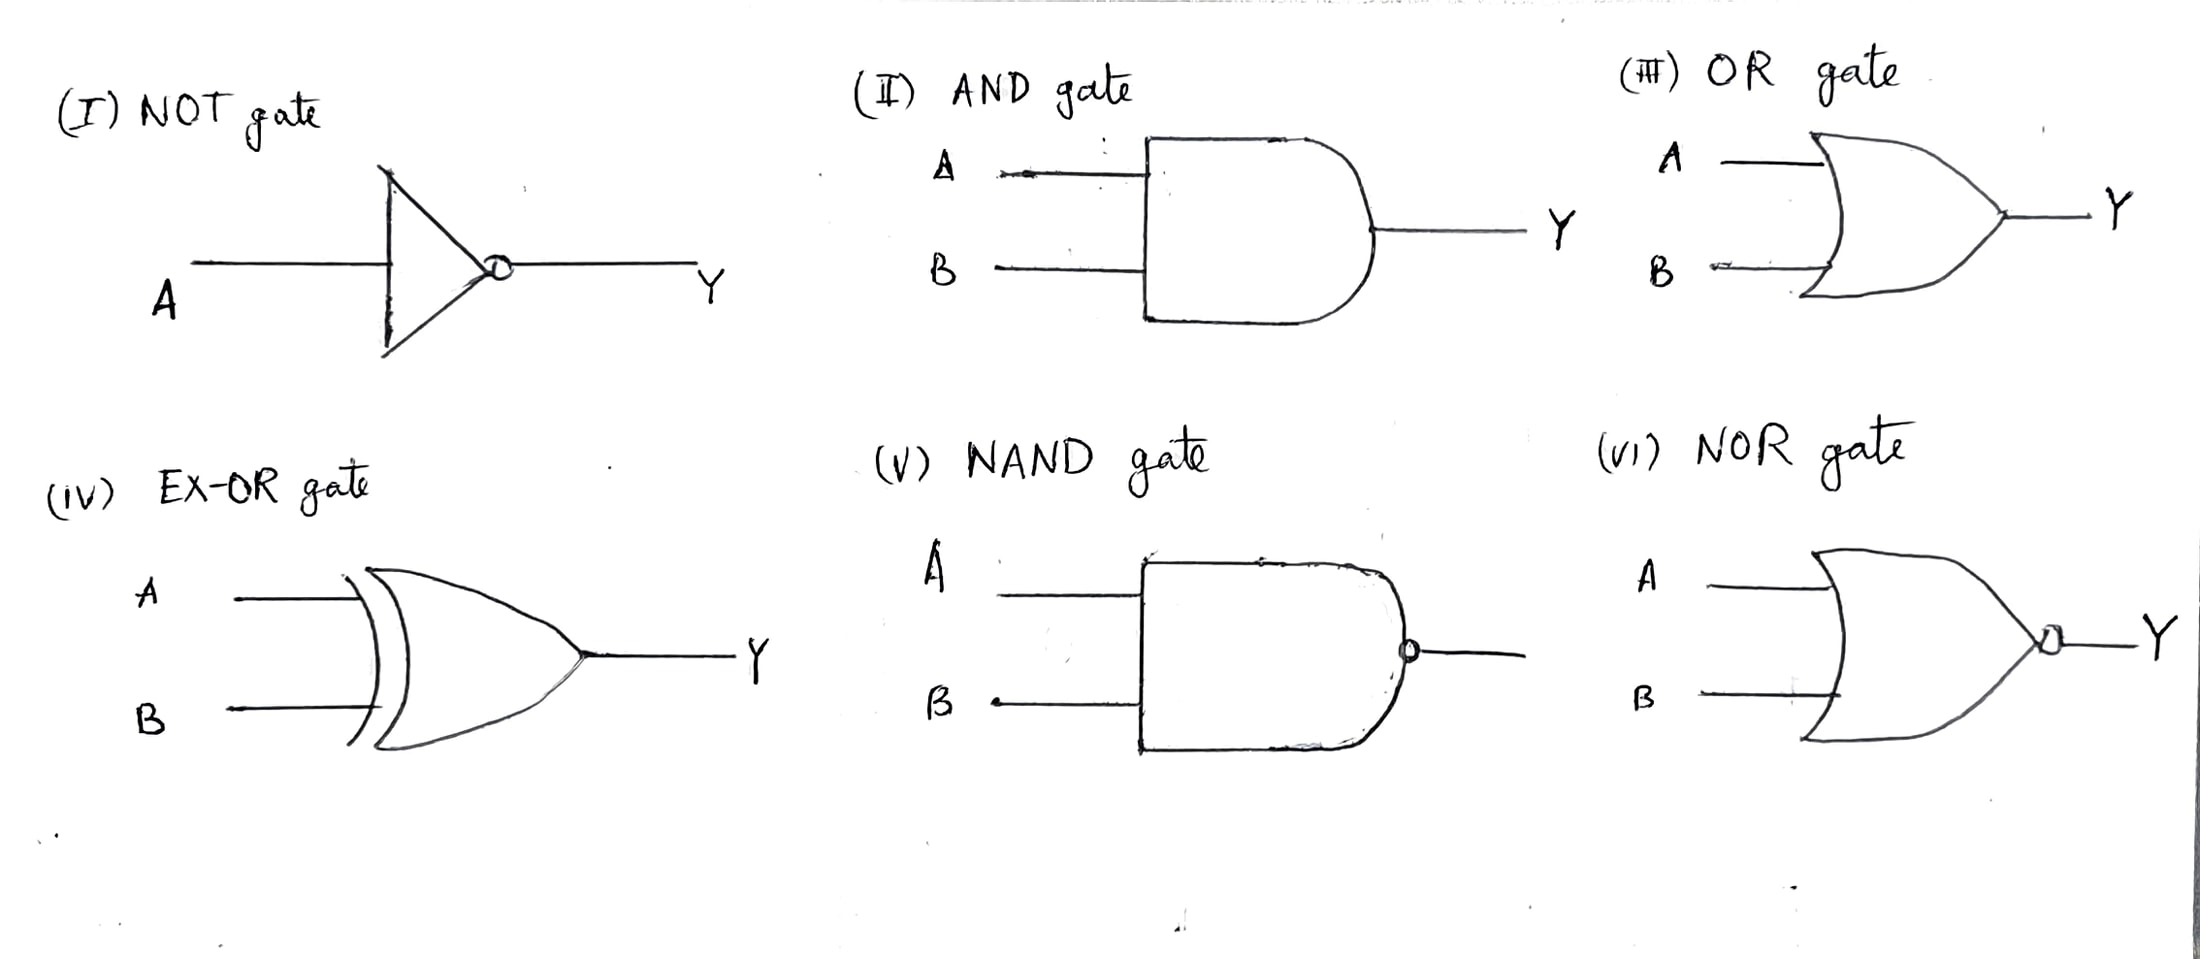
\includegraphics[scale = 0.2]{Documents/1615794012333.jpg}
\end{center}
\noindent
In propositional logic and Boolean algebra, \textbf{\emph{De Morgan's laws}} are a pair of transformation rules that are both valid rules of inference. The rules allow the expression of conjunctions and disjunctions purely in terms of each other via negation.
\newline
\noindent
In electrical and computer engineering, the laws are stated as follows:
\begin{enumerate}
    \item $\overline{A \cdot B} \equiv \overline{A} + \overline{B}$
    \item $\overline{A + B} \equiv \overline{A} \cdot \overline{B}$
\end{enumerate}
where 
\begin{itemize}
    \item $\cdot$ is the logical AND operator.
    \item $+$ is the logical OR operator.
    \item and the $\overline{overbar}$ is the logical NOT operator of what is underneath the overbar.
\end{itemize}
\begin{center}
    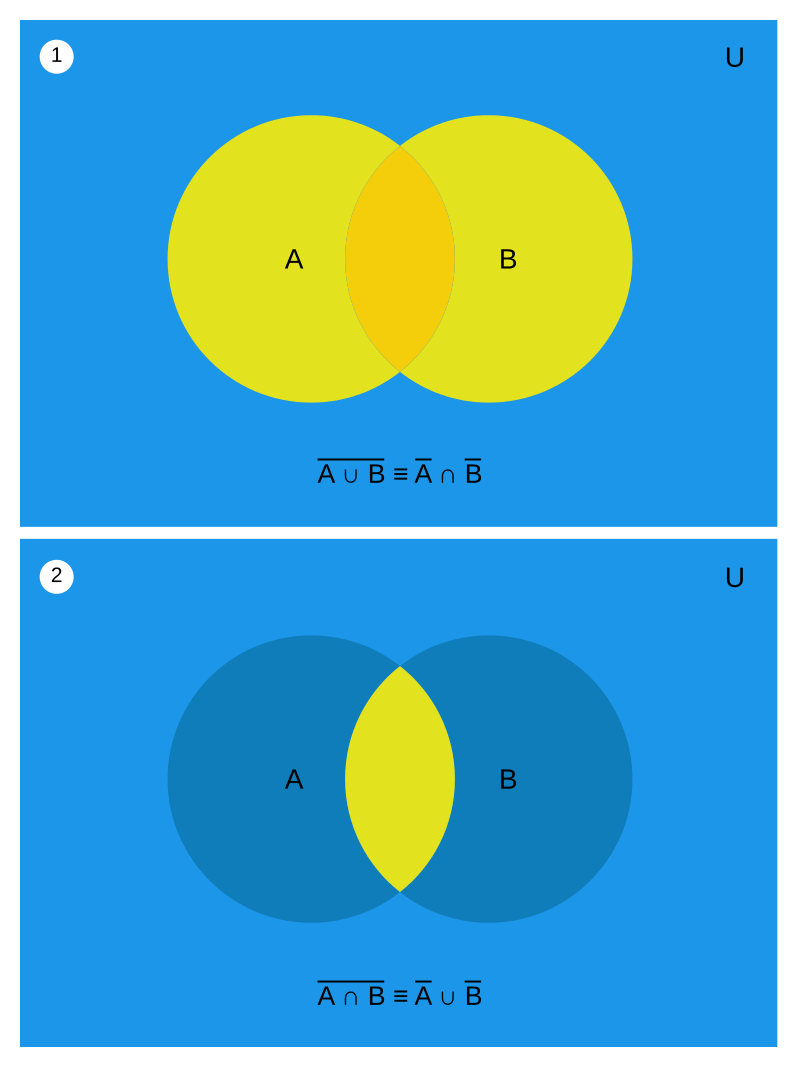
\includegraphics[scale = 0.16]{Documents/800px-Demorganlaws.svg.png}
\end{center}
\begin{center}
    \textbf{De Morgan's Law represented using Venn diagrams}
\end{center}
\clearpage
\section{Circuit Diagrams}
\begin{center}
    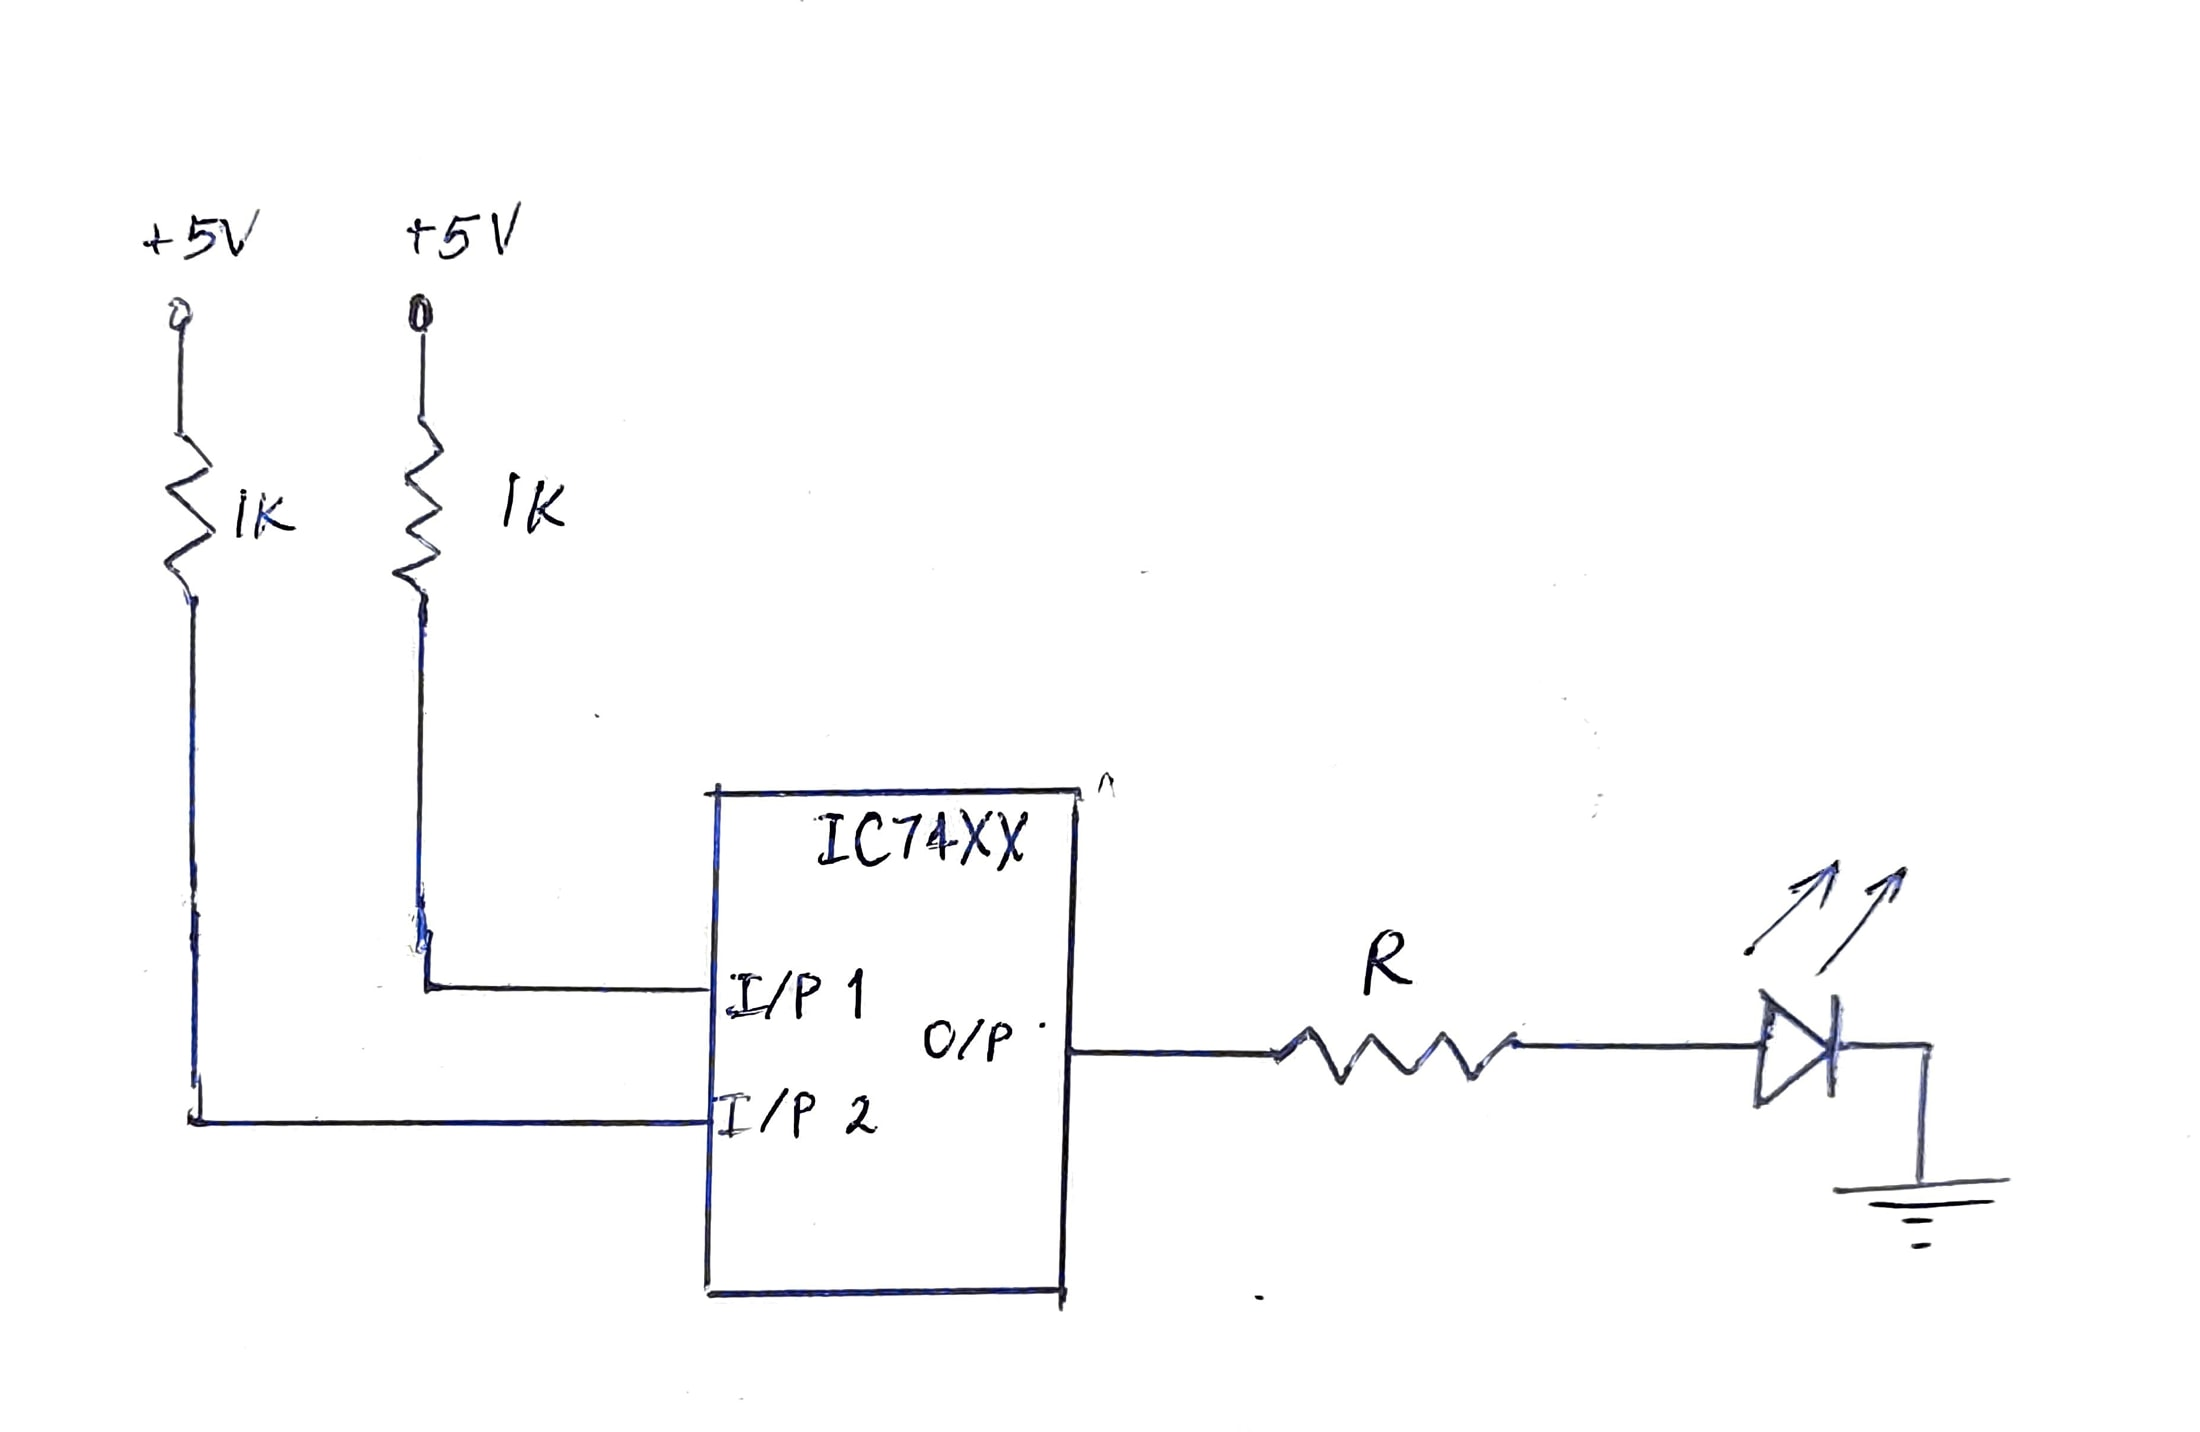
\includegraphics[scale = 0.11]{Documents/logicgate_1.jpg}
\end{center}
\begin{center}
    \textbf{General configuration for Logic Gate circuits}
\end{center}
\begin{center}
    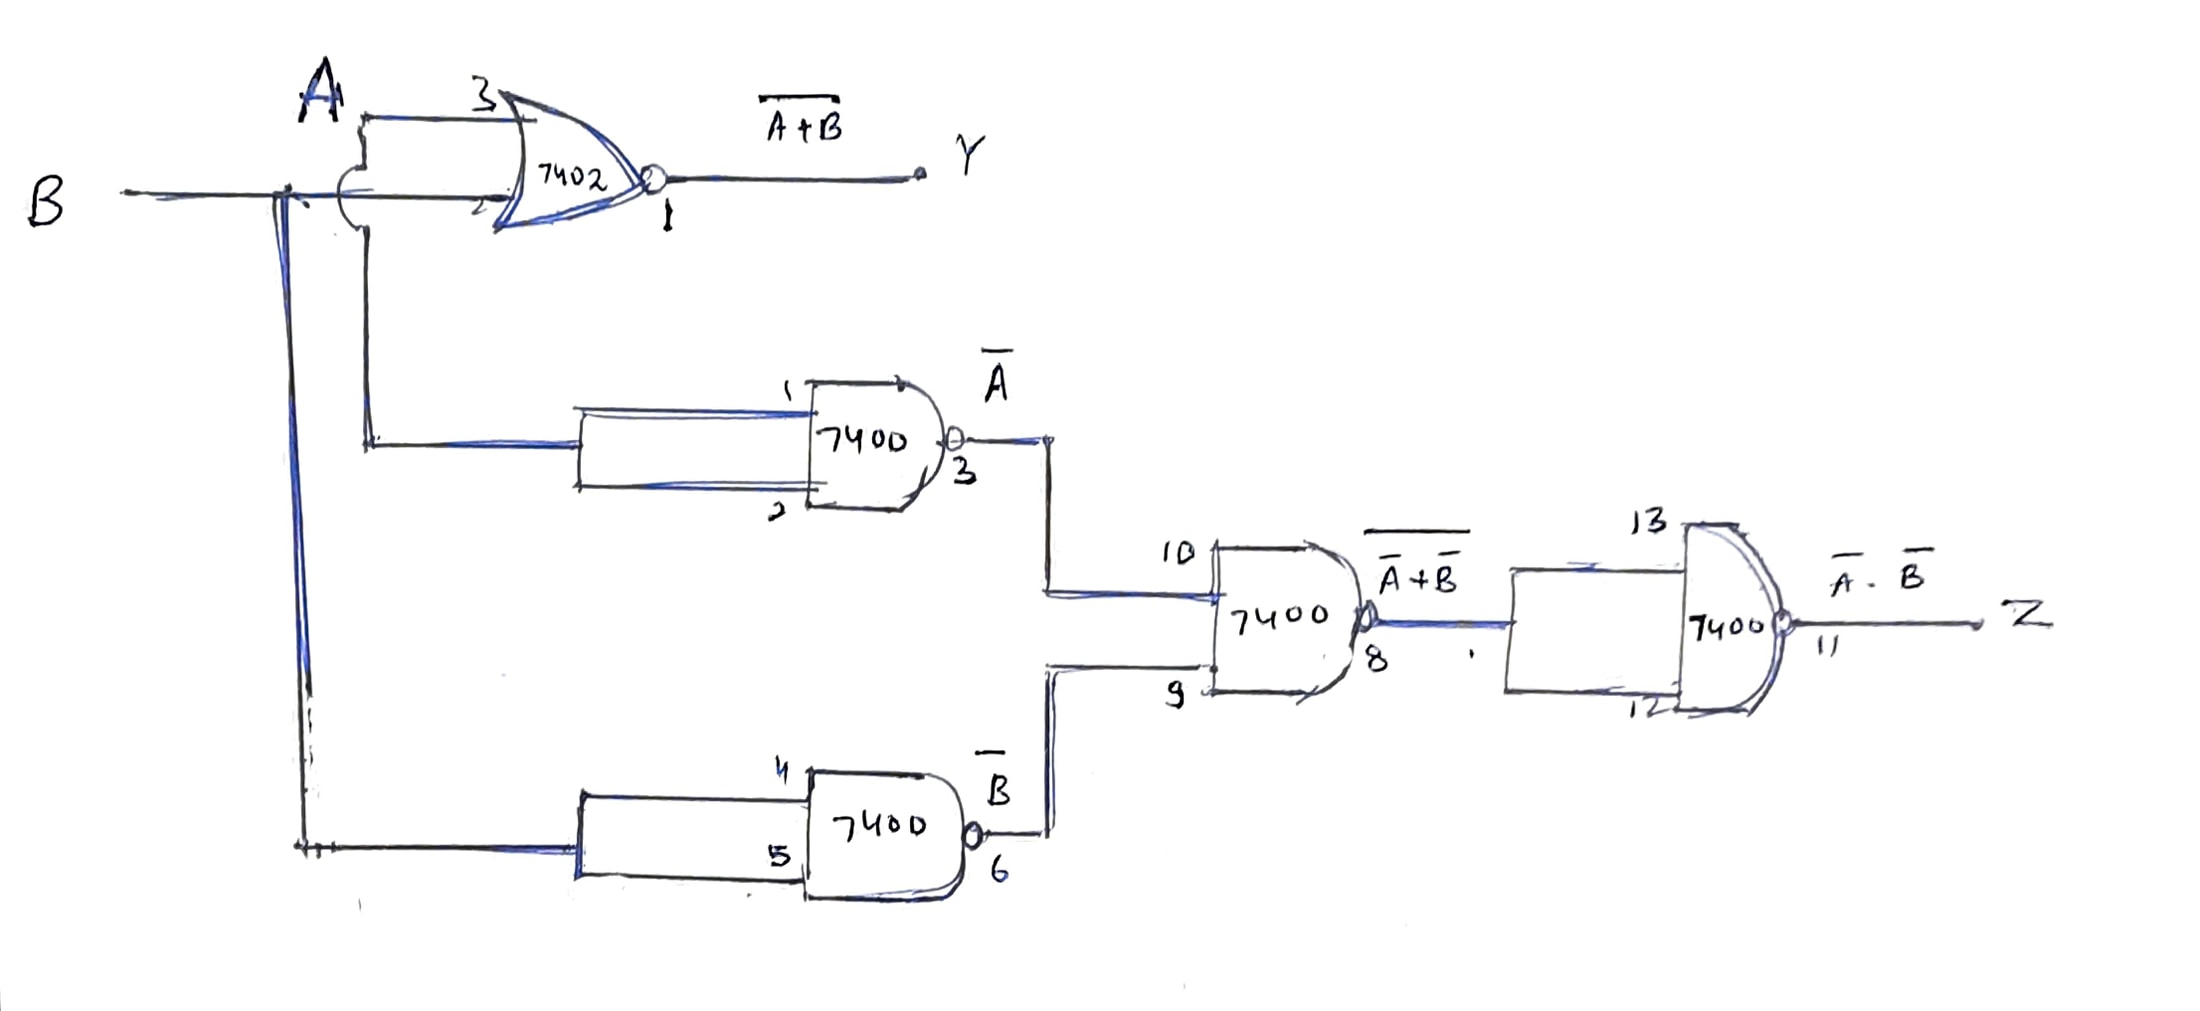
\includegraphics[scale = 0.16]{Documents/demorgans1_1.jpg}
\end{center}
\begin{center}
    \textbf{De Morgan's Law: $\overline{A + B} \equiv \overline{A} \cdot \overline{B}$}
\end{center}
\begin{center}
    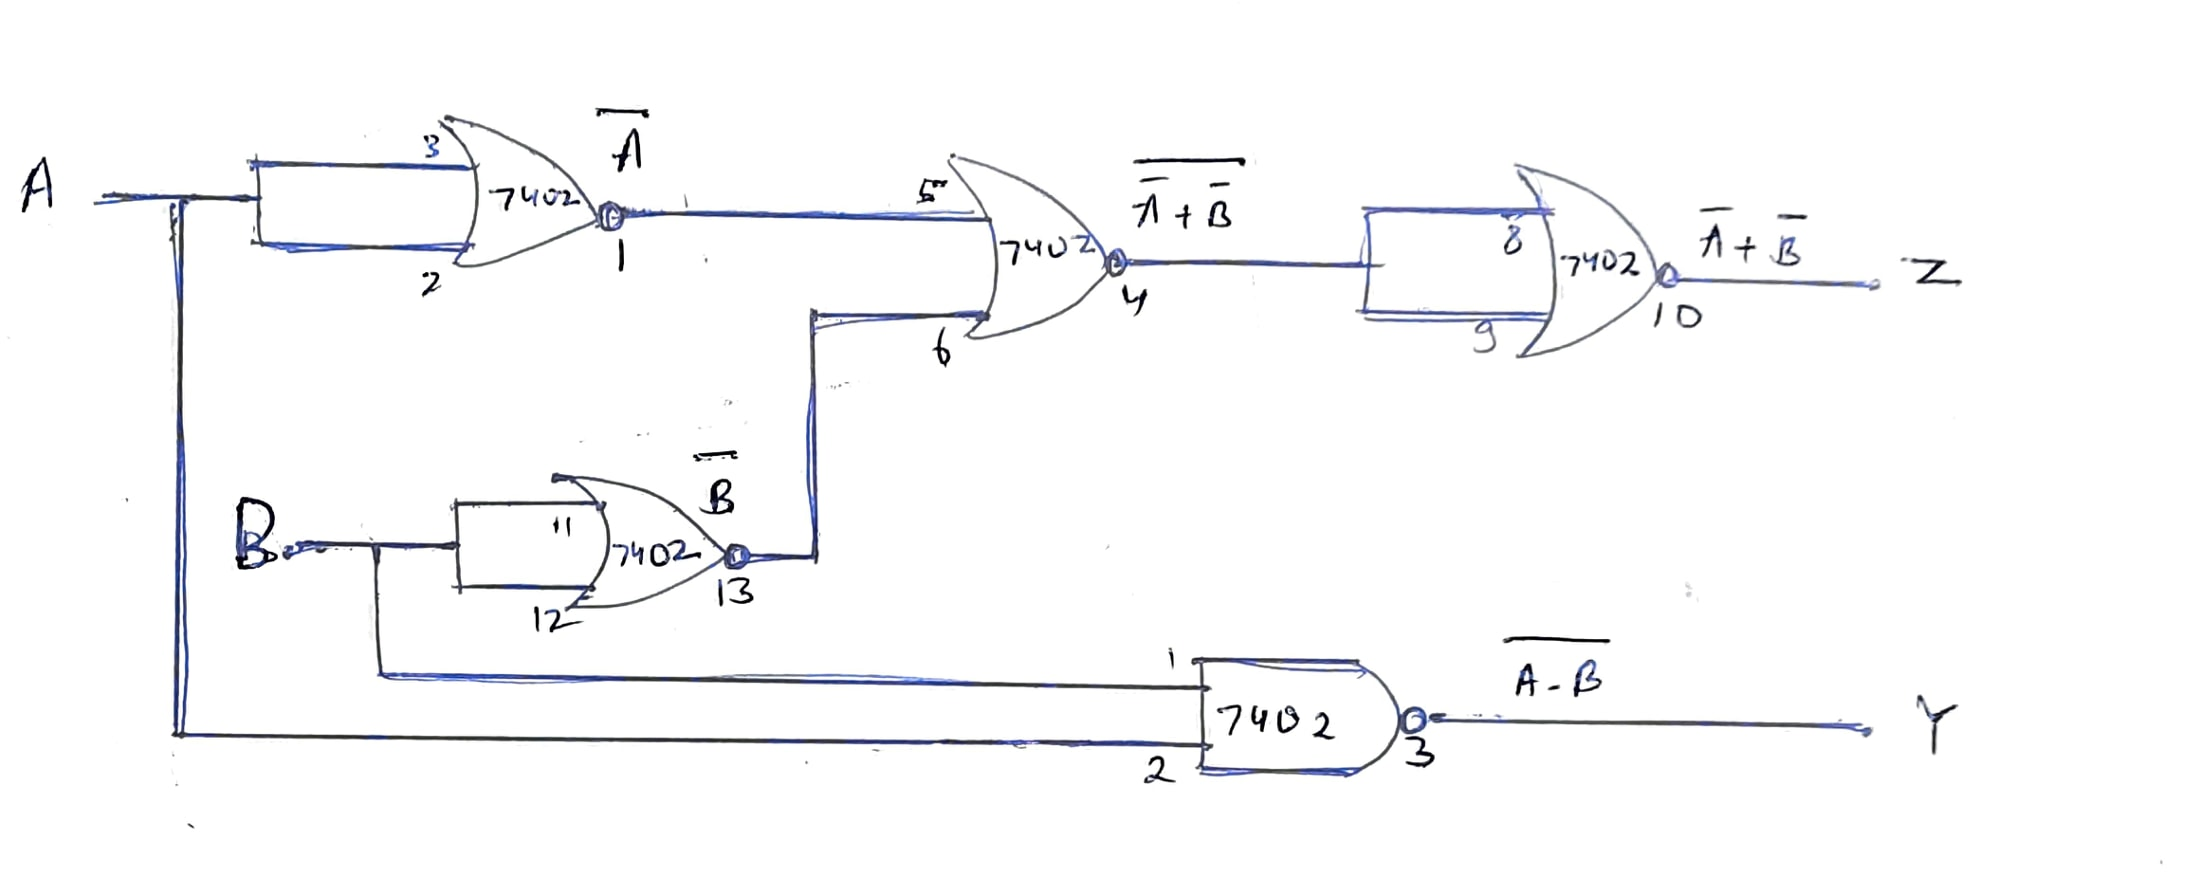
\includegraphics[scale = 0.16]{Documents/demorgans2_1.jpg}
\end{center}
\begin{center}
    \textbf{De Morgan's Law: $\overline{A \cdot B} \equiv \overline{A} + \overline{B}$}
\end{center}
\section{Observations}
\begin{center}
    \textbf{Verification of the Logical Operators}
\end{center}
\begin{center}
    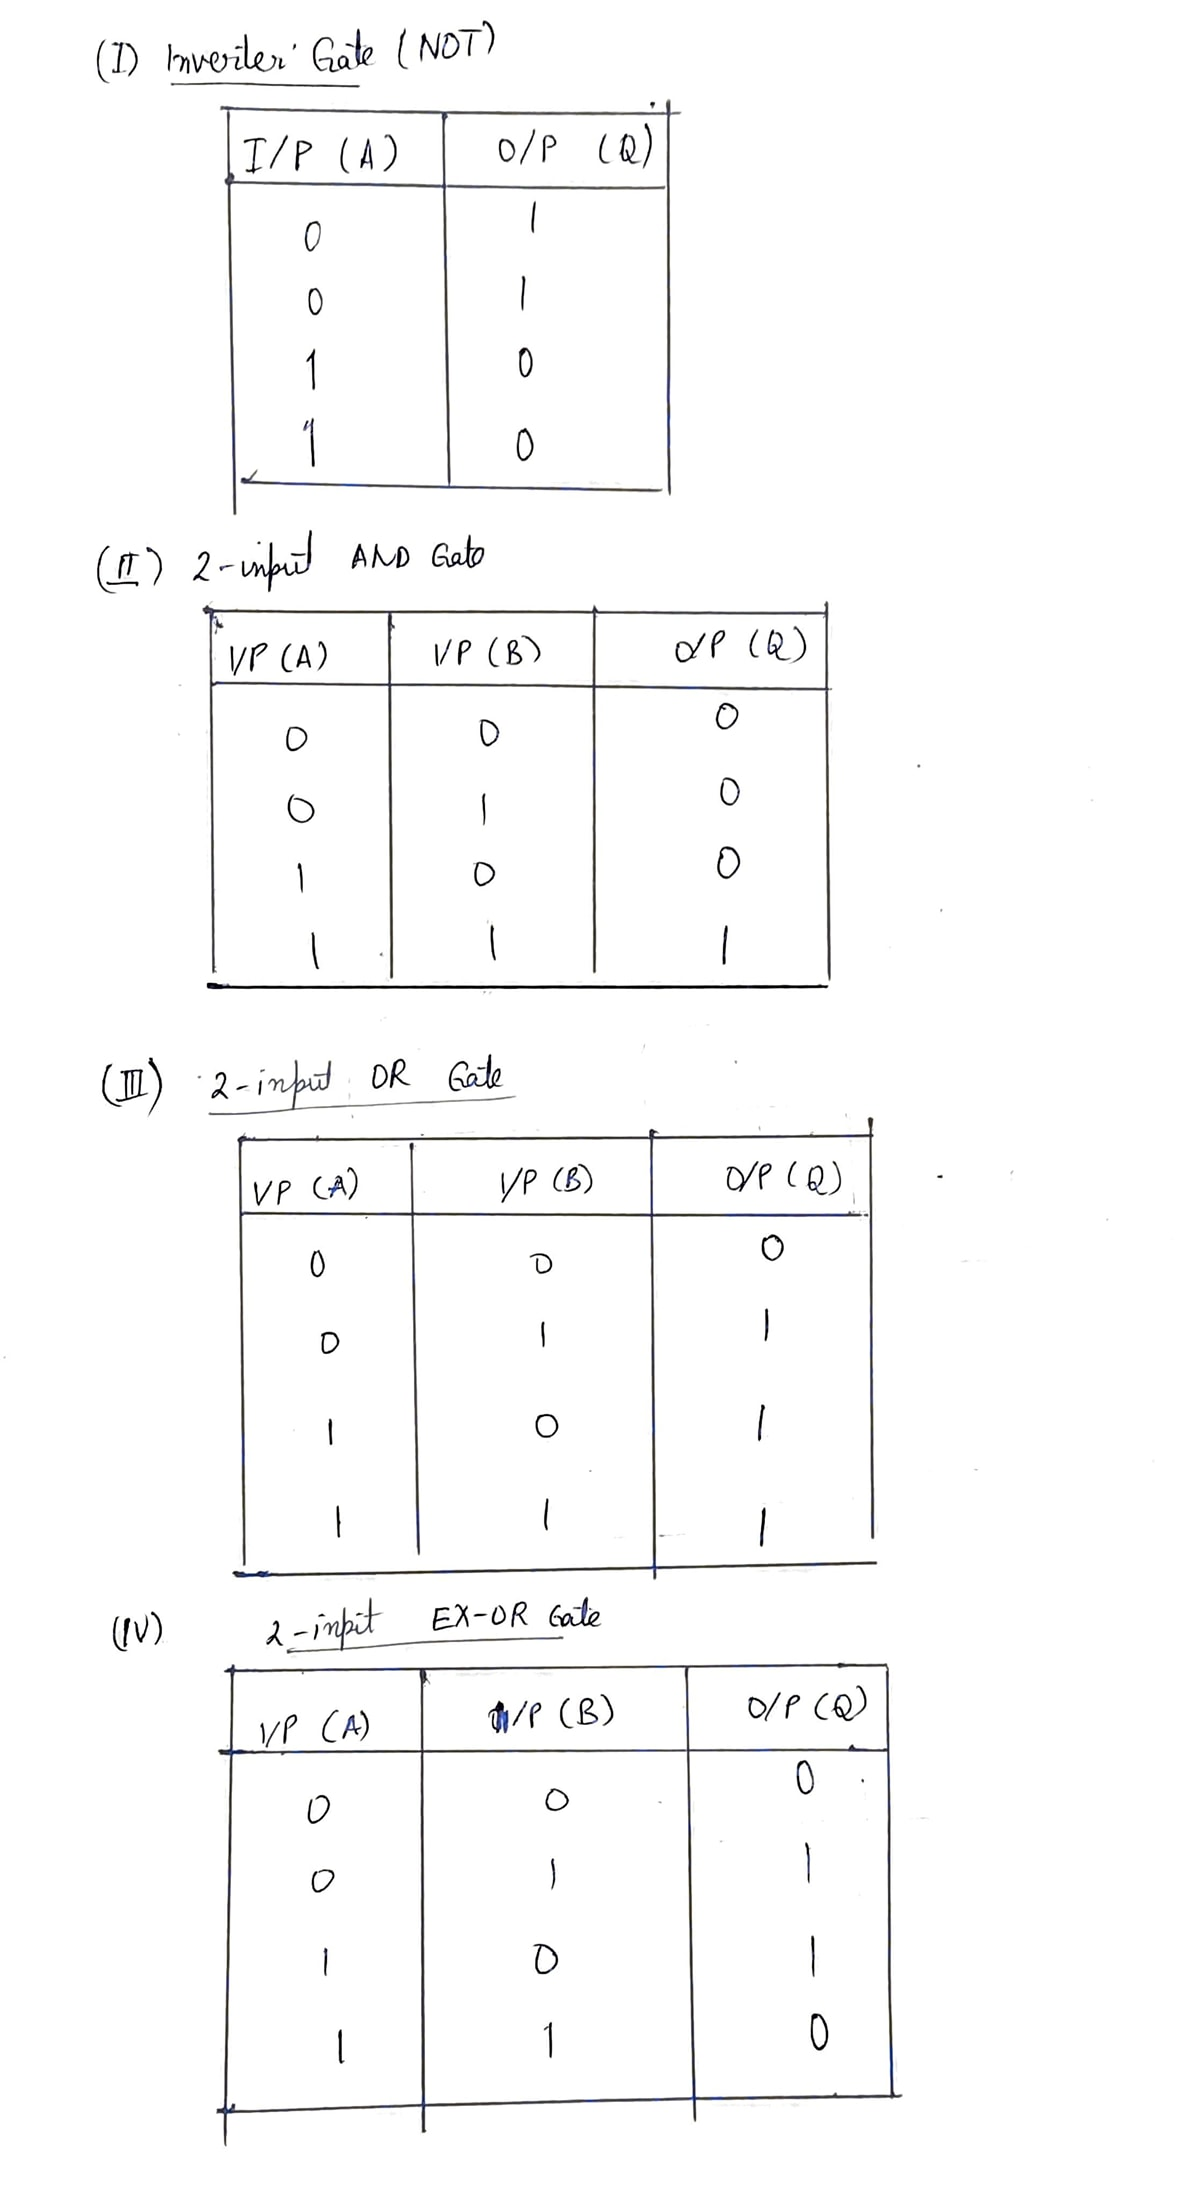
\includegraphics[scale = 0.25]{Documents/exp4tab1_1.jpg}
\end{center}
\clearpage
\begin{center}
    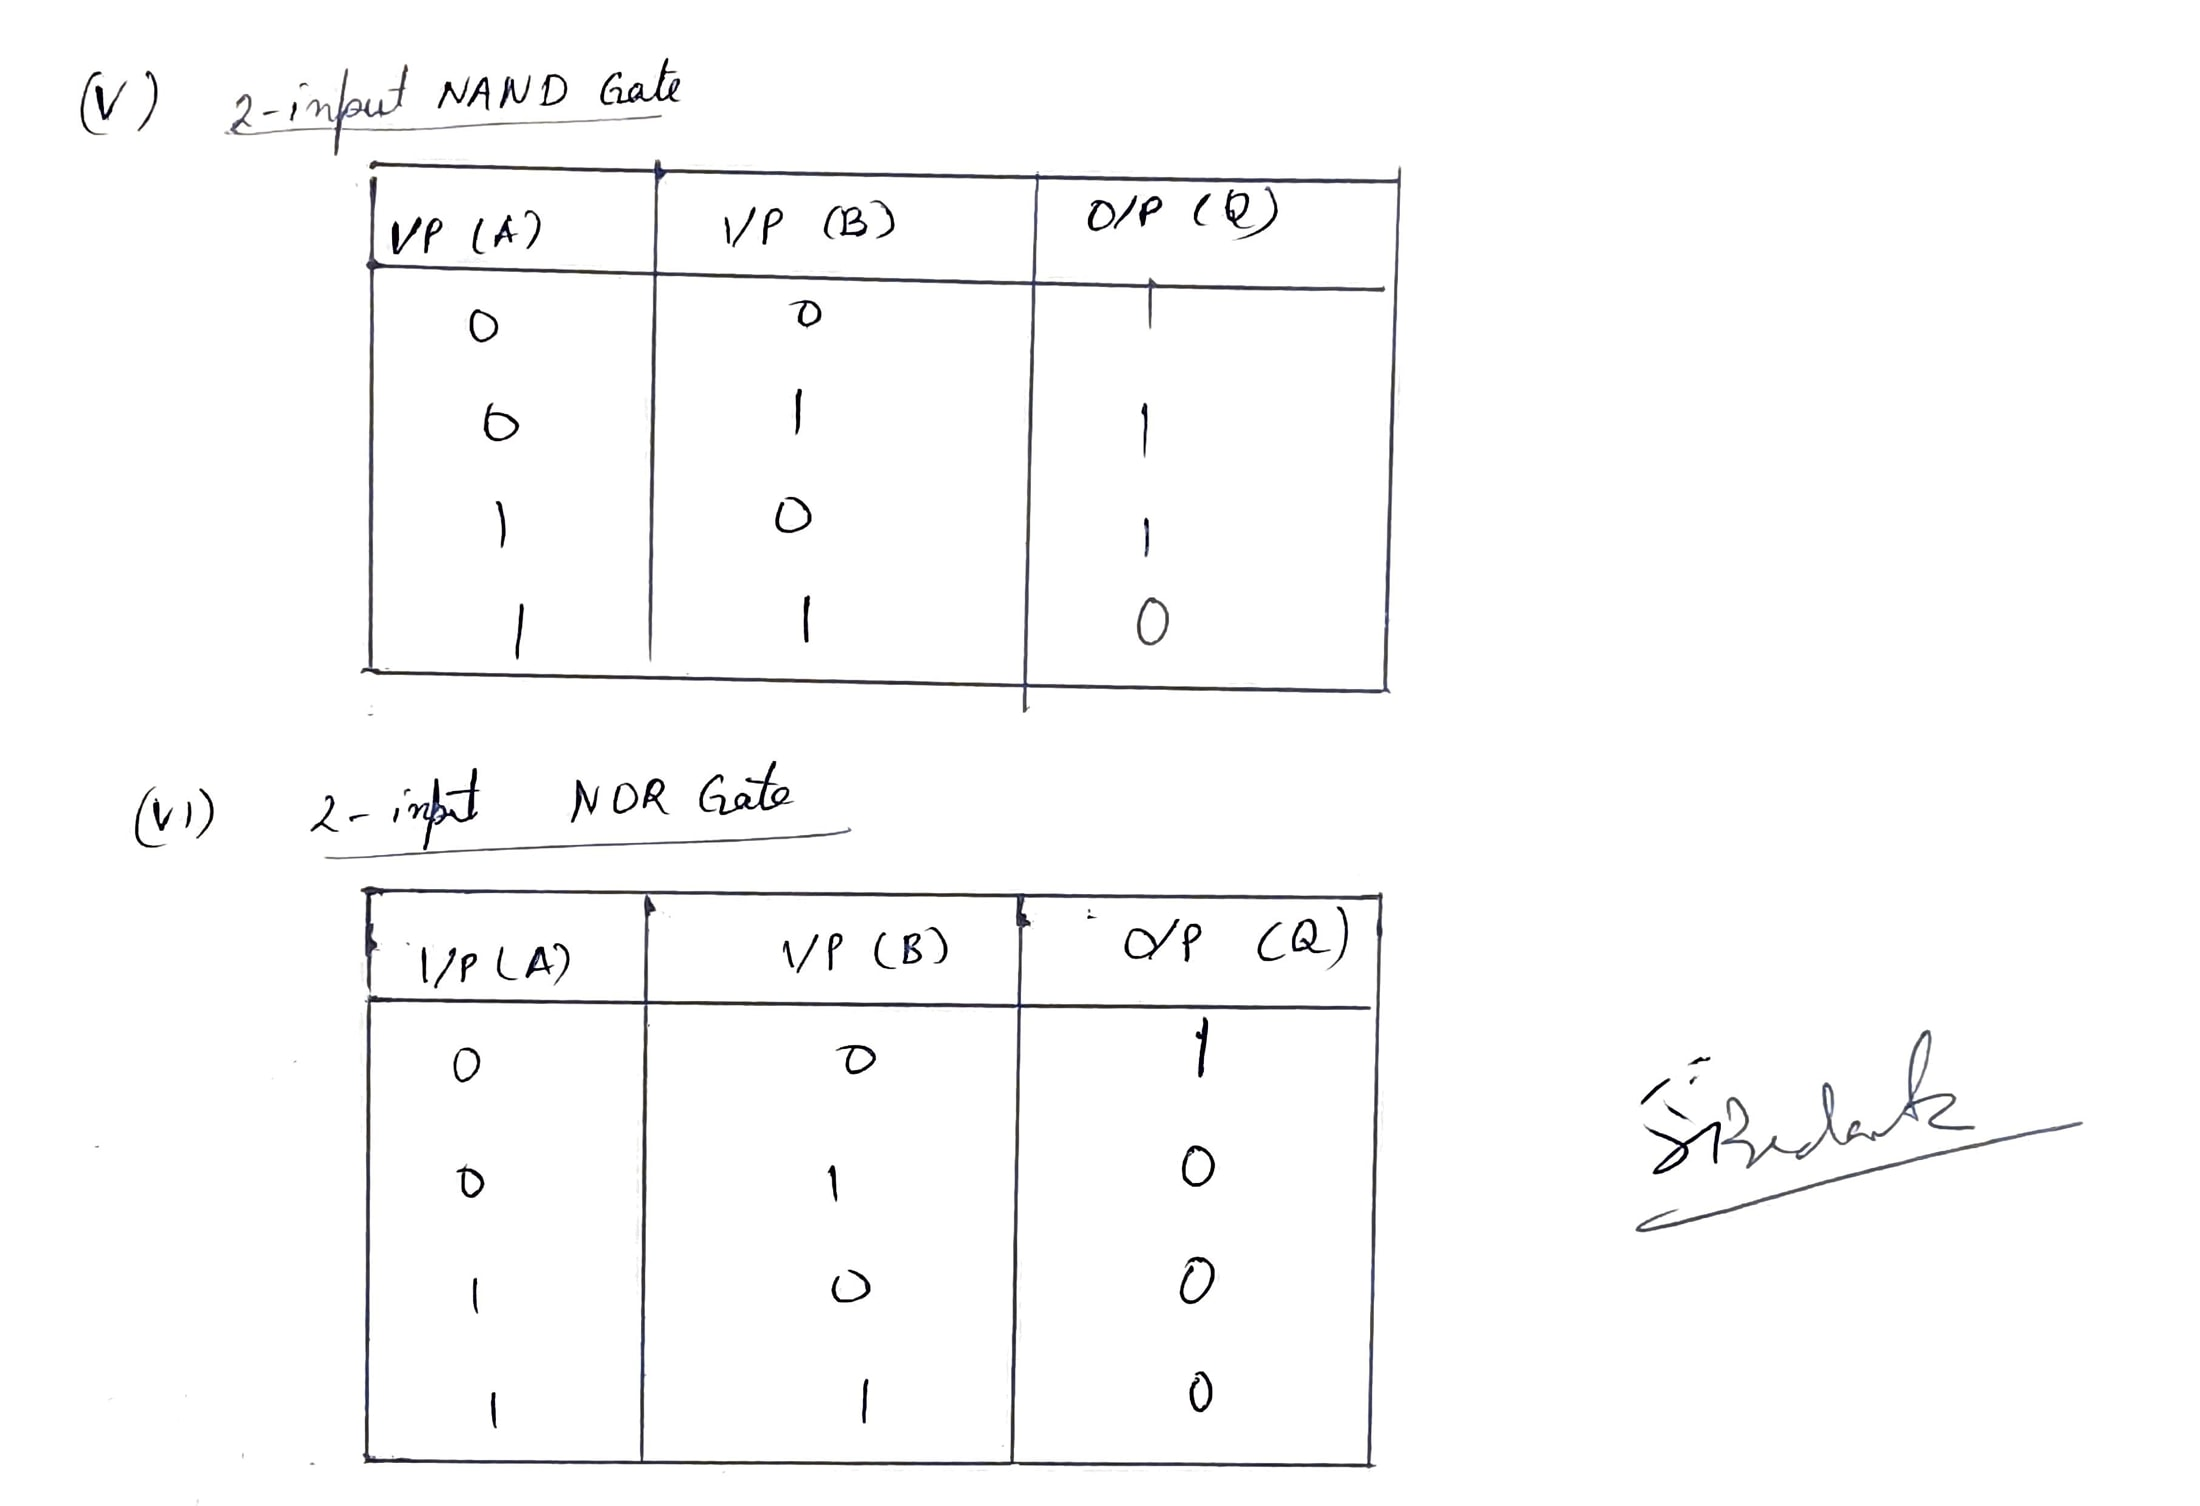
\includegraphics[scale = 0.2]{Documents/exp4tab1.5_1.jpg}
\end{center}
\begin{center}
    \textbf{Verification of De Morgan's Laws}
\end{center}
\begin{center}
    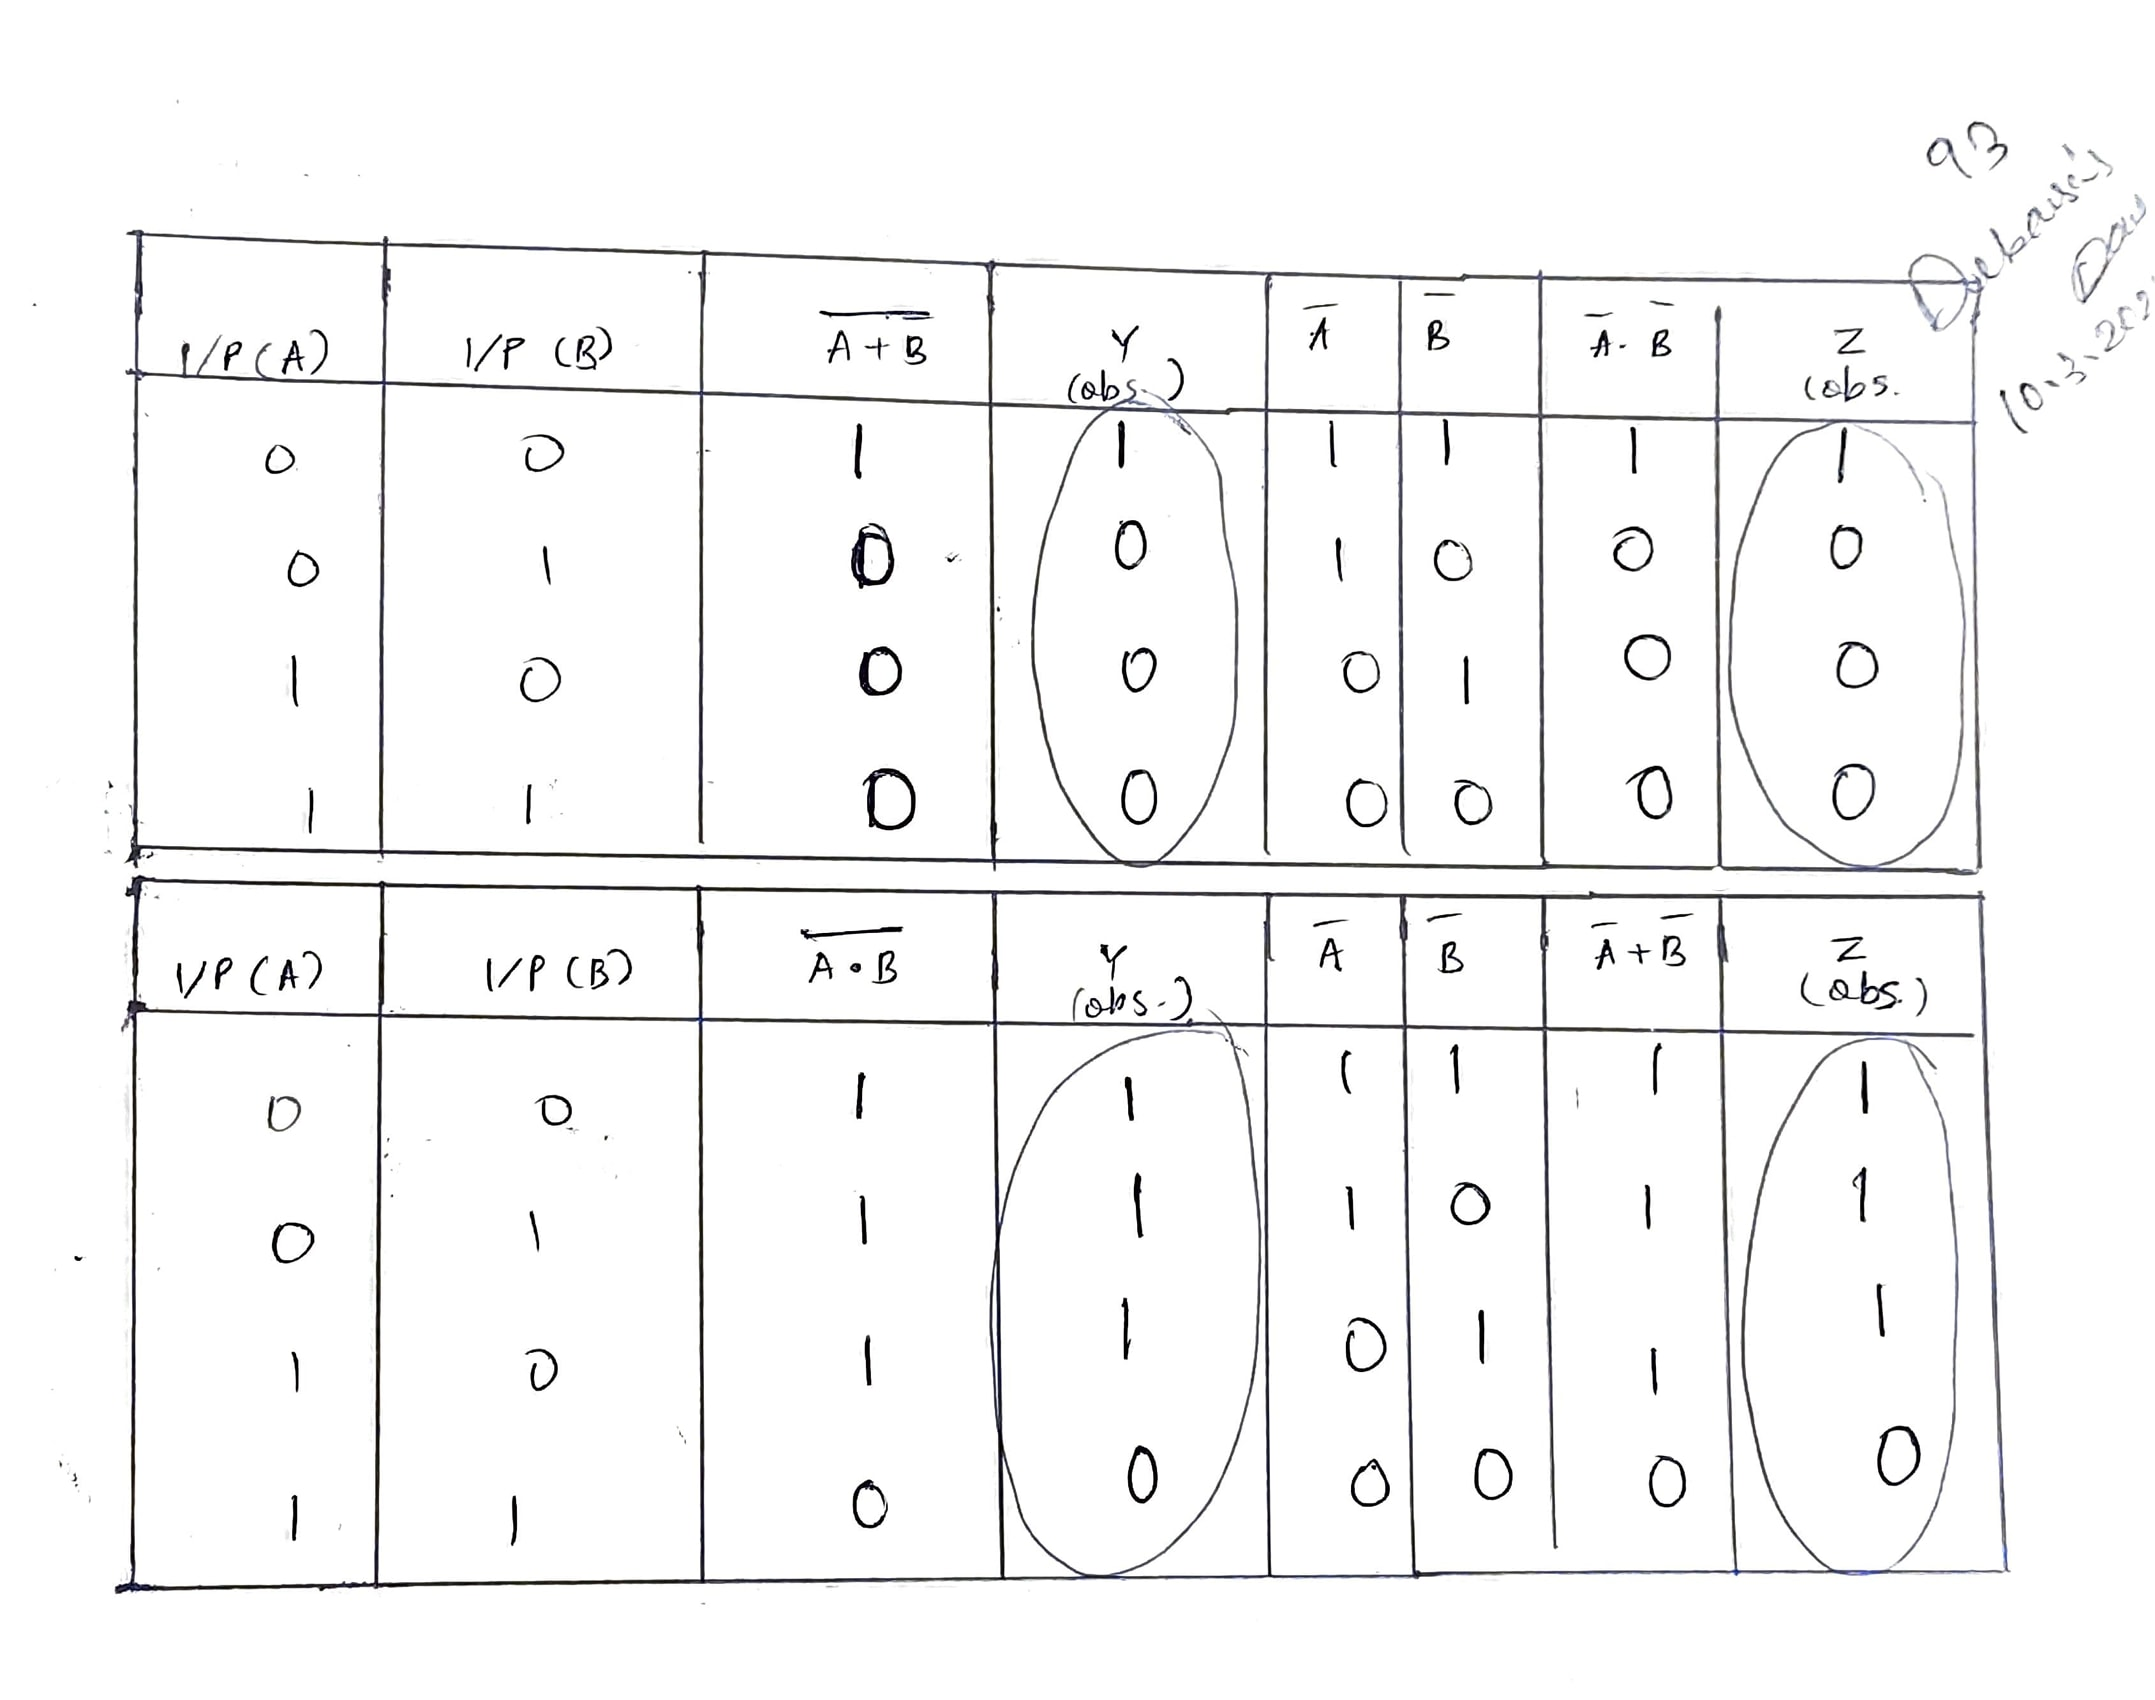
\includegraphics[scale = 0.16]{Documents/exp4tab2_1.jpg}
\end{center}
\section{Results}
\begin{enumerate}
    \item The logic gate truth tables are obtained as enumerated under Observations section
    \item The De Morgan's laws are verified.
\end{enumerate}
\section{Discussions}
\begin{enumerate}
    \item Logic gates can be used in various areas in the daily life.
    \item The logic gates are basically used in circuits involving computation and processing. They carry out the logical operations in every CPU architecture in computers.
    \item They are also used in push button switches, for example in door bells.
    \item They are used in the functioning of street lights.
    \item NAND Gates are used in Burglar alarms and buzzers.
    \item AND Gates are used to enable/inhibit the data transfer function.
\end{enumerate}
\section{Error Analysis}
\begin{enumerate}
    \item This experiment being a qualitative one, there are no errors per se.
    \item But we can note some precautions such as loose wiring leading to flickering of the LEDs (thus no conclusive "ON" or "OFF" inference.)
\end{enumerate}
\section{Conclusion}
\begin{enumerate}
    \item All results obtained are in accordance to the expectations.
\end{enumerate}